\documentclass[border=1mm]{standalone}

\usepackage{graphicx,tikz,tikz-layers}
\usetikzlibrary{decorations.markings,calc,positioning,arrows.meta}
% COLORS
\usepackage{xcolor}
\colorlet{myred}{red!80!black}
\colorlet{myblue}{blue!80!black}
\colorlet{mybluee}{myblue!80!black}
\colorlet{mygreen}{green!60!black}
\colorlet{myorange}{orange!70!red!60!black}
\colorlet{mydarkred}{red!30!black}
\colorlet{mydarkblue}{blue!40!black}
\colorlet{mydarkgreen}{green!30!black}


\begin{document}

\begin{tikzpicture}[
    font=\footnotesize,
    box/.style={draw, minimum width=1.2cm, minimum height=4cm, fill=myblue!15, rounded corners=3pt},
    patch/.style={minimum size=0.5cm},
    patch2/.style={minimum size=0.3cm},
    >={Latex[length=1.5mm, width=1.25mm]}
]

% Input image
\node[minimum size=2cm] (orig) at (0,0) {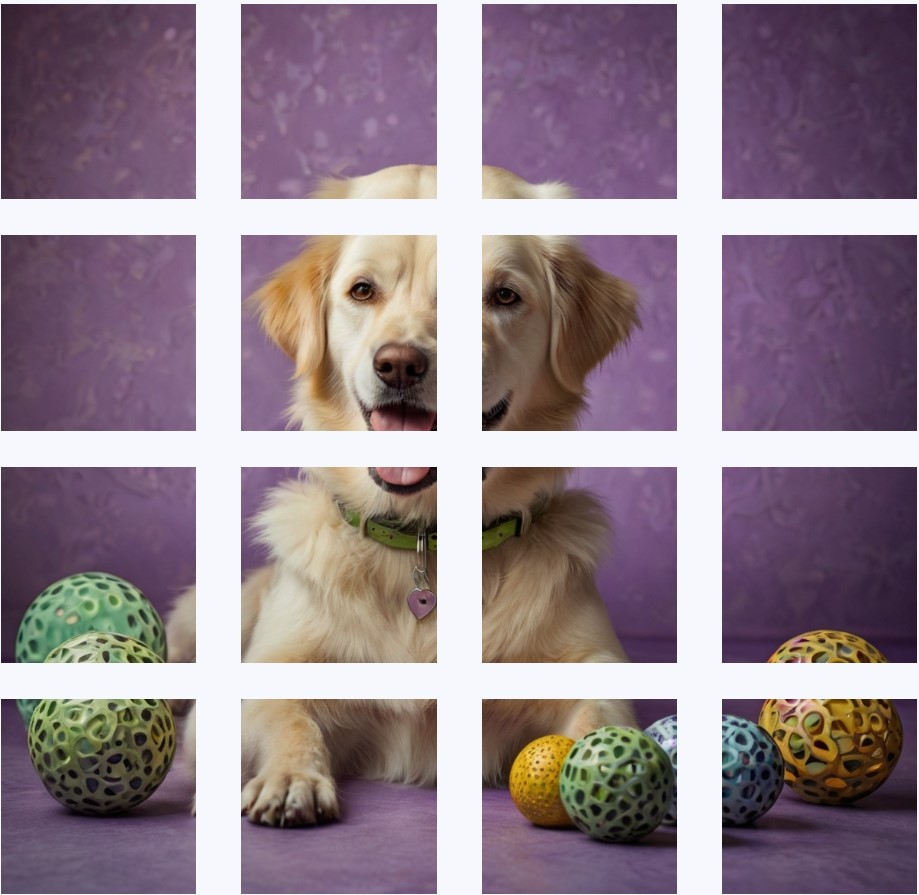
\includegraphics[width=2cm]{images/mosaic2/pdog.jpg}};

\node[fill=gray!50, draw,rectangle,minimum size=4.2mm, draw=gray!50, xshift =-0.26cm, yshift=0.25cm] {};
\node[fill=gray!50, draw,rectangle,minimum size=4.2mm, draw=gray!50, xshift =-0.26cm, yshift=0.75cm] {};
\node[fill=gray!50, draw,rectangle,minimum size=4.2mm, draw=gray!50, xshift =-0.26cm, yshift=-0.76cm] {};
\node[fill=gray!50, draw,rectangle,minimum size=4.2mm, draw=gray!50, xshift =0.78cm, yshift=0.25cm] {};
\node[fill=gray!50, draw,rectangle,minimum size=4.2mm, draw=gray!50, xshift =-0.78cm, yshift=-7.22] {};
\node[fill=gray!50, draw,rectangle,minimum size=4.2mm, draw=gray!50, xshift =0.78cm, yshift=0.75cm] {};
\node[fill=gray!50, draw,rectangle,minimum size=4.2mm, draw=gray!50, xshift =0.26cm, yshift=0.75cm] {};
\node[fill=gray!50, draw,rectangle,minimum size=4.2mm, draw=gray!50, xshift =0.78cm, yshift=-0.26cm] {};


\node[patch] (p1) at (2.3,2.1) {
\includegraphics[width=0.5cm]{tikz/images/mosaic2/00.jpg}};
\node[patch, below=-0.15cm of p1] (p2) {
\includegraphics[width=0.5cm]{tikz/images/mosaic2/01.jpg}};
\node[patch, below=-0.15cm of p2] (p3) {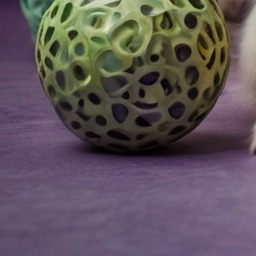
\includegraphics[width=0.5cm]{tikz/images/mosaic2/03.jpg}};
\node[patch, below=-0.15cm of p3] (p4) {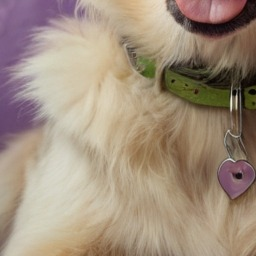
\includegraphics[width=0.5cm]{tikz/images/mosaic2/12.jpg}};
\node[patch, below=-0.15cm of p4] (p5) {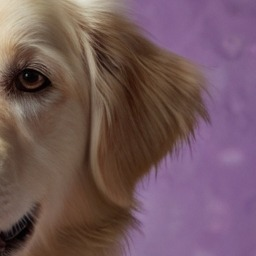
\includegraphics[width=0.5cm]{tikz/images/mosaic2/21.jpg}};
\node[patch, below=-0.15cm of p5] (p6) {
\includegraphics[width=0.5cm]{tikz/images/mosaic2/22.jpg}};
\node[patch, below=-0.15cm of p6] (p7) {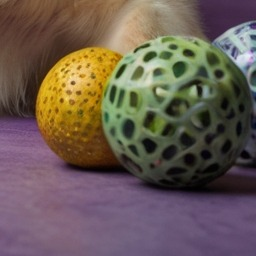
\includegraphics[width=0.5cm]{tikz/images/mosaic2/23.jpg}};
\node[patch, below=-0.15cm of p7] (p8) {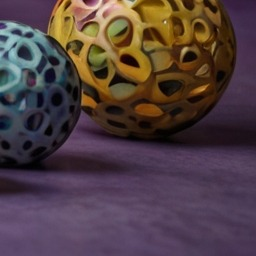
\includegraphics[width=0.5cm]{tikz/images/mosaic2/33.jpg}};

% Input patches column
% \foreach \i in {0,...,7} {
%     \node[patch] (p\i) at (3,-\i*0.6) {\includegraphics[width=0.5cm]{images/mosaic2/0\i.jpg}};
% }

% Encoder
\node[box] (encoder) at (3.45,-0.005) {Encoder};

\node[patch, fill=mybluee!20] (p1) at (4.6,2.1) {};
\node[patch, fill=mybluee!20, below=0.0851cm of p1] (p2) {};
\node[patch, fill=mybluee!20, below=0.0851cm of p2] (p3) {};
\node[patch, fill=mybluee!20, below=0.0851cm of p3] (p4) {};
\node[patch, fill=mybluee!20, below=0.0851cm of p4] (p5) {};
\node[patch, fill=mybluee!20, below=0.0851cm of p5] (p6) {};
\node[patch, fill=mybluee!20, below=0.0851cm of p6] (p7) {};
\node[patch, fill=mybluee!20, below=0.0851cm of p7] (p8) {};


\node[patch2, fill=gray!30] (p1) at (6,3) {};
\node[patch2, fill=gray!30, below=0.0851cm of p1] (p2) {};
\node[patch2, fill=mybluee!20, below=0.0851cm of p2] (p3) {};
\node[patch2, fill=gray!30, below=0.0851cm of p3] (p4) {};
\node[patch2, fill=gray!30, below=0.0851cm of p4] (p5) {};
\node[patch2, fill=gray!30, below=0.0851cm of p5] (p6) {};
\node[patch2, fill=mybluee!20, below=0.0851cm of p6] (p7) {};
\node[patch2, fill=gray!30, below=0.0851cm of p7] (p8) {};
\node[patch2, fill=gray!30, below=0.0851cm of p8] (p9) {};
\node[patch2, fill=mybluee!20, below=0.0851cm of p9] (p10) {};
\node[patch2, fill=mybluee!20, below=0.0851cm of p10] (p11) {};
\node[patch2, fill=gray!30, below=0.0851cm of p11] (p12) {};
\node[patch2, below=0.0851cm of p12] (p16) {...};
\node[patch2, fill=mybluee!20, below=0.0851cm of p16] (p17) {};
\node[patch2, fill=gray!30, below=0.0851cm of p17] (p18) {};
\node[patch2, fill=gray!30, below=0.0851cm of p18] (p19) {};


% Decoder
\node[box] (decoder) at (7.07,0) {Decoder};



\node[patch2, fill=myred!20] (p1) at (8.15,3) {};
\node[patch2, fill=myred!20, below=0.0851cm of p1] (p2) {};
\node[patch2, fill=myred!20, below=0.0851cm of p2] (p3) {};
\node[patch2, fill=myred!20, below=0.0851cm of p3] (p4) {};
\node[patch2, fill=myred!20, below=0.0851cm of p4] (p5) {};
\node[patch2, fill=myred!20, below=0.0851cm of p5] (p6) {};
\node[patch2, fill=myred!20, below=0.0851cm of p6] (p7) {};
\node[patch2, fill=myred!20, below=0.0851cm of p7] (p8) {};
\node[patch2, fill=myred!20, below=0.0851cm of p8] (p9) {};
\node[patch2, fill=myred!20, below=0.0851cm of p9] (p10) {};
\node[patch2, fill=myred!20, below=0.0851cm of p10] (p11) {};
\node[patch2, fill=myred!20, below=0.0851cm of p11] (p12) {};
\node[patch2, below=0.0851cm of p12] (p16) {...};
\node[patch2, fill=myred!20, below=0.0851cm of p16] (p17) {};
\node[patch2, fill=myred!20, below=0.0851cm of p17] (p18) {};
\node[patch2, fill=myred!20, below=0.0851cm of p18] (p19) {};

% Output image
\node[minimum size=2cm] (target) at (10.35,0) {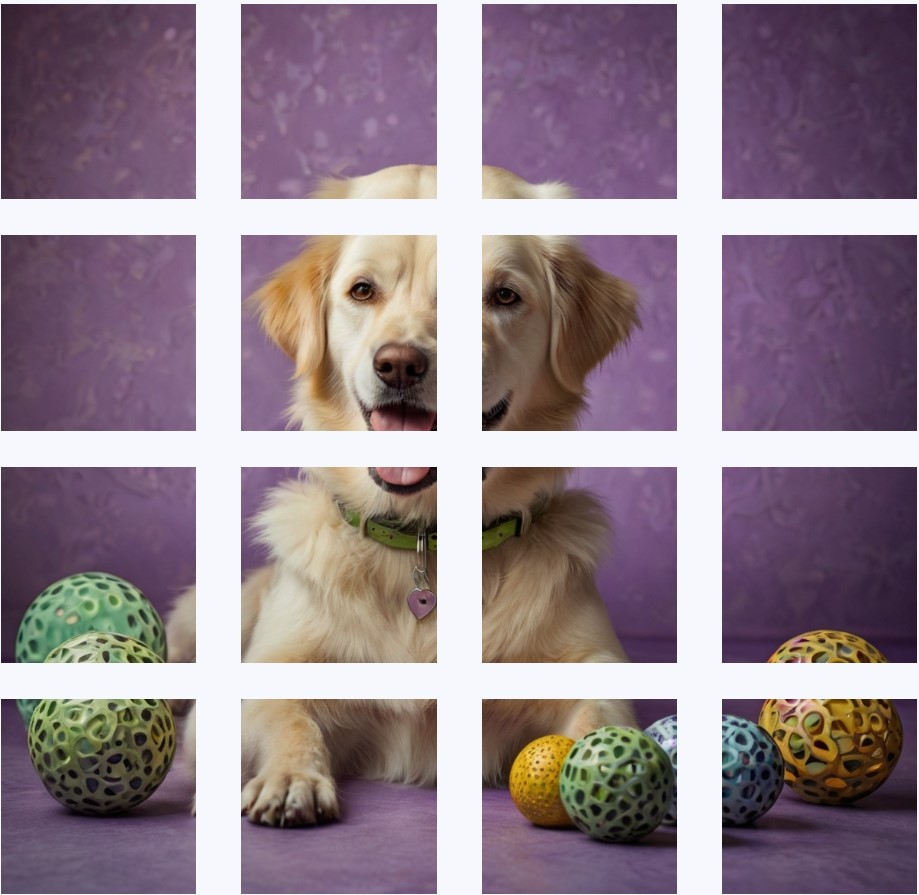
\includegraphics[width=2cm]{images/mosaic2/pdog}};

% Arrows
\draw[->] (orig.east) -- +(0.8,0);
\draw[->] (5,-0.005) -- +(0.7,0);
\draw[->] (8.5,-0.005) -- +(0.7,0);

\end{tikzpicture}

\end{document}